\chapter{OpenFOAM}
\label{ch:OpenFOAM}
In the previous chapter we looked at the \MP method as first proposed by original authors.
Since the goal of this master thesis is to use the \MP method implemented in \OF we will now take a closer look at how it is currently implemented.
The \OF version used in this \texttt{v2412}.
\begin{itemize}
    \item Use for simulation
\end{itemize}

\section{Introduction to OpenFOAM}
\begin{itemize}
    \item Open source toolbox for CFD simulation
    \item Three steps: Pre-processing (Utilities, Meshing Tools), Solving (MP-PIC), Post-processing (Paraview, other)
    \item Show different files:
    \begin{itemize}
        \item blockMeshDict
        \item controlDict
        \item fvSchemes
    \end{itemize}
\end{itemize}

\section{\MP method in OpenFOAM}

The \MP method in \OF can be roughly structured in the following diagram:

\begin{figure}
\centering
    \begin{tikzpicture}[node distance =2cm]
    \tikzset{stretch/.initial=.5}
        \tikzstyle{startstop} = [rectangle, rounded corners, minimum width=3cm, minimum height=1cm,text centered, draw=black]
        \tikzstyle{io} = [trapezium, trapezium left angle=70, trapezium right angle=110, minimum width=3cm, minimum height=1cm, text centered, draw=black, fill=blue!30]
        \tikzstyle{process} = [rectangle, minimum width=3cm, minimum height=1cm, text centered, draw=black]
        \tikzstyle{decision} = [diamond, minimum width=3cm, minimum height=1cm, text centered, draw=black, fill=green!30]
        \tikzstyle{arrow} = [thick,->,>=stealth]
        \node (start) [startstop] {\parbox{5cm}{\centering create Mesh, initialize Fields \\ apply Boundary conditions}};
        %\node (createMesh) [decision, right of=start,xshift = 6cm] {\texttt{createFields.H}};
        \node (in1) [process, below of=start] {Still run time?};
        \node (endTime) [startstop, right of=in1, xshift = 3cm] {Stop};
        \node (dec1) [process, below of=in1] {Evaluate kinematic and dynamic viscosity};
        %\node (pro1) [process, below of=dec1] {Tridiagonal solver for $\alpha_p$ and $\alpha_f \rho_f$};
        % \draw[thick,->] ($(pro1.north east)$) .. controls +(1.9,1) and +(1.9,-1).. node[right] {\parbox{2.5cm}{Iterate until convergence}}  ($(pro1.south east)$);
        %\path let \p1 = ($(pro1.north east)$), \p2 = ($(pro1.south east)$) in node[draw, red, anchor=west] t (\p1) {Top Right}node[draw, blue, anchor=west] at (\p2) {Bottom Right};
        \node (pro2) [process, below of=dec1] {Evolve kinematic cloud};
        \node (pro3) [process, below of=pro2] {Interpolate to Eulerian mesh / build source terms};
        \node (stop) [process, below of = pro3] {\texttt{PIMPLE} loop};
        \draw[arrow] (start) -- (in1);
        \draw[arrow] (in1) -- node[anchor=south] {no} (endTime);
        \draw[arrow] (in1) -- node[anchor = west] {yes} (dec1);
        \draw[arrow] (dec1) -- (pro2);
        \draw[arrow] (pro2) -- (pro3);
        %\draw[arrow] (pro1) -- (pro2);
        %\draw[arrow] (pro2) -- (dec1);
        \draw[arrow] (pro3) -- (stop);
        %\draw[thick,->] (stop.west) .. controls +(-2.5,1.5) and +(-2.5,0)..  (start.west);
        \draw[thick,->,rounded corners]
  (stop.west) --
  ($ ({stop.west}|-{stop.west}) + (-4,0) $) -- % move left from stop.west
  ($ ({stop.west}|-{in1.west}) + (-4,0) $) -- % vertical, x fixed from stop.west
  (in1.west);
    \end{tikzpicture}
\end{figure}

In the following we will go into detail for each step.

\subsection{Create Fields}
\subsection{Continuous Phase Transport}

\subsection{Evolve Kinematic Cloud}
Evolving the kinematic cloud is done by calling \lstinline|kinematicCloud.evolve();| in the \lstinline|MPPICFoam.C| file. This calls the \lstinline|solve| method from the Lagrangian kinematic cloud class.
It can be split into roughly four steps. First the kinematic cloud is prepared in the \lstinline|preEvolve| step and relevant data is cashed. Then the particles are moved in \lstinline|evolveCloud|. 
If the solver is coupled the new velocity is offset with the old velocity, which is done in \lstinline|coupled|.
Lastly, in \lstinline|postEvolve| cashed data is released and relevant data is written out.
This represents the standard Lagragian kinematic cloud evolving.
The \MP method is worked into the \lstinline|evolveCloud| method, more specifically into \lstinline|motion|.
In the following flow chart \ref{fig:FCEvoleCloud} we outline which methods are called when the kinematic cloud is evolved.
We will look at each step in more detail in the following.


\FloatBarrier
\begin{figure}
    \centering
\begin{tikzpicture}[
    node distance=12mm and 6mm,
    every node/.style={font=\small},
    box/.style={draw, rounded corners, minimum width=26mm, minimum height=10mm, align=center},
    lane/.style={draw, rounded corners, fill=gray!10, minimum width=42mm, minimum height=85mm},
    pre/.style={box, fill=MidnightBlue!20},
    evo/.style={box, fill=RedViolet!20},
    coup/.style={box, fill=ForestGreen!20},
    post/.style={box, fill=YellowOrange!20},
    title/.style={font=\bfseries},
    scale = 0.9,
    transform shape
]

% --- Swimlanes ---
\node[lane] (L1) {};
\node[lane, right=of L1] (L2) {};
\node[lane, right=of L2] (L3) {};
\node[lane, right=of L3] (L4) {};

\node[title, above=1mm of L1] {pre evolve};
\node[title, above=1mm of L2] {evolve cloud};
\node[title, above=1mm of L3] {coupled};
\node[title, above=1mm of L4] {post evolve};

% --- Left lane ---
%\node[pre] (pre) at (L1.center |- [yshift=-42.5mm]L1.north) {preEvolve()};
\node[pre] (pre)
  at ([yshift=-42.5mm] L1.center |- L1.north) {preEvolve()};

% --- Evolve cloud lane ---
\node[evo] (e1) at ([yshift=-9.5mm] L2.center |- L2.north) {evolveCloud()};
\node[evo, below=of e1] (e2) {resetSourceTerms()};
\node[evo, below=of e2] (e3) {inject()};
\node[evo, below=of e3] (e4) {motion()};

% --- Coupled lane ---
\node[coup] (c1) at ([yshift=-31.5mm] L3.center |- L3.north) {coupled?};
\node[coup, below=of c1] (c2) {relaxSources()};

% --- Post lane ---
\node[post] (p1) at ([yshift=-42.5mm] L4.center |- L4.north) {postEvolve()};
%\node[post, below=of p1] (p2) {stochasticCollisionModel()};

% --- Arrows ---
%\draw[->, thick] (pre.east) -- (e1.west);
\draw[->,rounded corners]
  (pre.east) --
  ($ ({pre.east}|-{pre.east}) + (1.1,0) $) -- % move left from stop.west
  ($ ({pre.east}|-{e1.west}) + (1.1,0) $) -- % vertical, x fixed from stop.west
  (e1.west);



\draw[->] (e1) -- (e2);
\draw[->] (e2) -- (e3);
\draw[->] (e3) -- (e4);

%\draw[->, thick] (e4.east) -- (c1.west);
\draw[->,rounded corners]
  (e4.east) --
  ($ ({e4.east}|-{e4.east}) + (1.1,0) $) -- % move left from stop.west
  ($ ({e4.east}|-{c1.west}) + (1.1,0) $) -- % vertical, x fixed from stop.west
  (c1.west);


\draw[->] (c1) -- node[right]{Yes} (c2);
%\draw[->] (c2.east) -- (p1.west);

%\draw[->] (c1.east) -- node[above]{No} (p1.west);
\draw[->,rounded corners]
  (c1.east) -- node[above]{No \text{   }}
  ($ ({c1.east}|-{c1.east}) + (1.1,0) $) -- % move left from stop.west
  ($ ({c1.east}|-{p1.west}) + (1.1,0) $) -- % vertical, x fixed from stop.west
  (p1.west);

\draw[->,rounded corners]
  (c2.east) --
  ($ ({c2.east}|-{c2.east}) + (1.1,0) $) -- % move left from stop.west
  ($ ({c2.east}|-{p1.west}) + (1.1,0) $) -- % vertical, x fixed from stop.west
  (p1.west);
  %\draw[thick,->,rounded corners]
  
  % (stop.west) --
  % ($ ({stop.west}|-{stop.west}) + (-4,0) $) -- % move left from stop.west
  % ($ ({stop.west}|-{in1.west}) + (-4,0) $) -- % vertical, x fixed from stop.west
  % (in1.west);


%\draw[->] (p1) -- (p2);
 \end{tikzpicture}
 \caption{Flow chart of the solve method in the Lagrangian kinematic cloud class.}
\label{fig:FCEvoleCloud}
 \end{figure}
\FloatBarrier

\todo{Flow chart nochmal als Text? (Bin stark dagegen das liest doch eh niemand)}
\subsubsection{preEvolve}
The \lstinline|preEvolve| prepares for the movement of the particles by caching important properties.
First, the mesh validity is checked.
Next Eulerian fields are cached for efficient memory usage and properties from the Eulerian mesh are later used to update particle positions.
The damping and packing models are prepared and properties needed to run them later are cashed.
\ifcode
\begin{lstlisting}[firstline = 782, caption=in KinematicCloud.C]
    template<cklass CloudType>
void Foam::KinematicCloud<CloudType>::preEvolve
(
    const typename parcelType::trackingData& td
)
{
    // force calculation of mesh dimensions - needed for parallel runs
    // with topology change due to lazy evaluation of valid mesh dimensions
    label nGeometricD = mesh_.nGeometricD();

    Log_<< "\nSolving" << nGeometricD << "-D cloud " << this->name() << endl;

    this->dispersion().cacheFields(true);
    forces_.cacheFields(true);

    pAmbient_ = constProps_.dict().template
        getOrDefault<scalar>("pAmbient", pAmbient_);

    if (this->dampingModel().active() || this->packingModel().active())
    {
         const_cast<typename parcelType::trackingData&>(td).updateAverages(*this);
    }

    if (this->dampingModel().active())
    {
        this->dampingModel().cacheFields(true);
    }
    if (this->packingModel().active())
    {
        this->packingModel().cacheFields(true);
    }

    updateCellOccupancy();

    functions_.preEvolve(td);
}

\end{lstlisting}
\fi

\subsubsection{evolveCloud}
The method \lstinline|evolveCloud()| is what moves the particles along their trajectories. For details the code is included in the following listing \ref{code:evolveCloud}.
First the source terms are reset. The source terms that contribute to the continuous equations will be built after the kinematic cloud has evolved.
Because the \MP solver is transient, we will only look at the first part of the \lstinline|if| condition. 
Particles are injected in two steps.
To check whether injection of particles has taken place, the current cloud size is recorded.
First particles generated from films, e.g walls, are injected.
If necessary, cell occupancy is updated.
In the second step, particles are injected from inlets.
Properties such as the velocity, size of the particles which is either pre-defined or given via a distribution etc. are set in this step from the tracking data \lstinline|td|.
The \lstinline|cloud.motion| command then moves the particles to their new time steps.
The motion method is defined in the \lstinline|MPPICCloud.C| file. This differs from the standard motion of the kinematic cloud. It will be discussed in the next section.
The stochastic collision model which is executed at the end of the evolve function is turned off in the \MP model, because a similar term is included in the return-to-isotropy damping model that is executed in \lstinline|motion|.

\ifcode
\begin{lstlisting}[firstnumber=221,caption=from kinematicCloud.C, label ={code:evolveCloud}]
    template<class CloudType>
template<class TrackCloudType>
void Foam::KinematicCloud<CloudType>::evolveCloud
(
    TrackCloudType& cloud,
    typename parcelType::trackingData& td
)
{
    if (solution_.coupled())
    {
        cloud.resetSourceTerms();
    }

    if (solution_.transient())
    {
        label preInjectionSize = this->size();

        this->surfaceFilm().inject(cloud);

        // Update the cellOccupancy if the size of the cloud has changed
        // during the injection.
        if (preInjectionSize != this->size())
        {
            updateCellOccupancy();
            preInjectionSize = this->size();
        }

        injectors_.inject(cloud, td);

        // Assume that motion will update the cellOccupancy as necessary
        // before it is required.
        cloud.motion(cloud, td);

        stochasticCollision().update(td, solution_.trackTime());
    }
    else
    {
//        this->surfaceFilm().injectSteadyState(cloud);

        injectors_.injectSteadyState(cloud, td, solution_.trackTime());

        td.part() = parcelType::trackingData::tpLinearTrack;
        CloudType::move(cloud, td, solution_.trackTime());
    }
}

\end{lstlisting}
\fi
\todo{lieber komplett lassen oder z.B. zweiten Teil (steady state) rausnehen}
\todo{trackTime ist nicht das selbe wie simulation time?}



\subsubsection{motion}
The method \lstinline|motion| is called from \lstinline|MPPICCloud.C| which differs from the previous code which was executed in \lstinline|KinematicCloud.C|. This is the core of the \MP method which was described in the previous section \ref{ch:MPPIC}. 
The outline of how the code is executed is shown in the following flow chart \ref{fig:FCMPPIC}.

\FloatBarrier
\begin{figure}[h!]
\centering
    \begin{tikzpicture}[node distance =2cm]
    \tikzset{stretch/.initial=.5}
        \tikzstyle{startstop} = [rectangle, rounded corners, minimum width=3cm, minimum height=1cm,text centered, draw=black]
        \tikzstyle{io} = [trapezium, trapezium left angle=70, trapezium right angle=110, minimum width=3cm, minimum height=1cm, text centered, draw=black, fill=blue!30]
        \tikzstyle{process} = [rectangle, minimum width=3cm, minimum height=1cm, text centered, draw=black]
        \tikzstyle{decision} = [diamond, minimum width=3cm, minimum height=1cm, text centered, draw=black, fill=green!30]
        \tikzstyle{arrow} = [thick,->,>=stealth]
        \node (start) [startstop] {Predict particle motion through particle forces (drag, gravity, etc)};
        \node (mv1) [process, below of=start] {Move Particles};
        \node (tau) [decission, below of = mv1] {$\tau < \tvar_{n+1}$};
        %\node (start1) [process, below of=start] {move particles according to forces};
        %\node (createMesh) [decision, right of=start,xshift = 6cm] {\texttt{createFields.H}};
        \node (in1) [process, below of=tau] {Switch Forces off};
        % \node (endTime) [startstop, right of=in1, xshift = 3cm] {Stop};
        \node (dec1) [process, below of=in1] {Apply collision damping model, move particles accordingly};
        %\node (pro2) [process, below of=dec1] {Move particles according to damping model};
        \node (pro3) [process, below of=dec1] {Apply packing model, move particles accordingly};
        %\node (pro4) [process, below of=pro3] {Move particles according to packing model};
        \node (pro5) [process, below of=pro3] {Apply return-to-isotropy damping model, move particles accordingly};
        %\node (pro6) [process, below of=pro5] {Move particles according to return-to-isotropy damping model};
        \node (stop) [process, below of = pro5] {Update cells/ turn forces back on};
        
        %\draw[arrow] (start) -- (start1);
        \draw[arrow] (start) -- (mv1);
        \draw[arrow] (mv1) -- (tau);
        \draw[arrow] (tau) -- node[anchor=west) {no}(in1);
        %\draw[arrow] (in1) -- node[anchor=south] {no} (endTime);
        %\draw[arrow] (in1) -- node[anchor = west] {yes} (dec1);
        \draw[arrow] (in1) --  (dec1);
        \draw[arrow] (dec1) -- (pro3);
        %\draw[arrow] (pro2) -- (pro3);
        \draw[arrow] (pro3) -- (pro5);
        %\draw[arrow] (pro4) -- (pro5);
        %\draw[arrow] (pro5) -- (pro6);
        %\draw[arrow] (pro1) -- (pro2);
        %\draw[arrow] (pro2) -- (dec1);
        \draw[arrow] (pro5) -- (stop);
        %\draw[thick,->] (stop.west) .. controls +(-2.5,1.5) and +(-2.5,0)..  (start.west);
        \draw[thick,->,rounded corners]
  (tau.east) --
  ($ ({tau.east}|-{tau.east}) + (6,0) $) -- node[anchor=east] {$\tau = $}
  ($ ({tau.east}|-{start.east}) + (6,0) $) -- 
  (start.east);
    \end{tikzpicture}
    \caption{Flow chart of \lstinline|motion| in \lstinline|MPPICCloud.C|.}
    \label{fig:FCMPPIC}
\end{figure}
\FloatBarrier
\Todo{Add time loop for particle time $\tau$}
In the previous section we defined the advanced time velocity in equation \ref{eq:errVel} as
\begin{equation*}
    \up^{n+1} = \dfrac{\up^n + \Delta \tvar \left[ \d_p \up^{n+1} - \dfrac{1}{\rp} \nabla \p_p^{n+1} - \dfrac{1}{\rp \pvf} \nabla \scs^{n+1} - \g \right]}{1 + \Delta \tvar \d} .
\end{equation*}
In the \MP implementation this is split up into two different terms.
\begin{align*}
    \up^{n+1} & = \tilde{\up}^{n+1} + \u_{p,\scs} \\
    \tilde{\up^{n+1}} &= \dfrac{\up^n + \Delta \tvar \left[ \d_p \up^{n+1} - \dfrac{1}{\rp} \nabla \p_p^{n+1} - \g \right]}{1 + \Delta \tvar \d} \qquad \u_{p,\scs} = - \dfrac{\Delta \tvar \nabla \scs}{\rp \pvf (1+\Delta \tvar \d)}
\end{align*}
In the first step only the first term that depends on particle forces is applied to the particles and they are moved accordingly.
The new particle positions are
\begin{equation*}
    \xp^{n+1} = \xp^n + \tilde{\up}^{n+1}.
\end{equation*}
Next the collision damping model is applied.
This is currently not properly implemented in \OF and will therefor not be discussed further here \cite{chimera}.

\Todo{stimmt zweiter Term?}
To model particle-particle interactions the particle normal stress is applied in the packing model.
Different models can be used here, as discussed in \ref{sec:particleNormalStress}.
To prevent unphysical behavior the packing model is only applied in certain cases \cite{MPInterpolation}.
The criterion depends on the relative velocity $\u_r$ which calculated the difference between the particle velocity and the averaged Eulerian particle velocity.
\begin{align*}
    \begin{cases}
        \u_{p,\scs} = - \dfrac{\Delta \tvar \nabla \scs}{\rp \pvf (1+\Delta \tvar \d)} & \text{if } \u_r \cdot \nabla \scs > 0  \\
        \u_{p,\scs} = 0 & \text{if } \u_r \cdot \nabla \scs \leq 0
    \end{cases} \qquad \u_r = \up - \overline{\up}
\end{align*}
To explain in which cases the particle normal stress model is applied we simplify the problem. In the following figure \ref{fig:WhenPacking} the particle normal stress model is applied for the cases marked in green.
For the figure we assume that the packed bed is on the left hand side and the particle volume fraction monotone increasing toward the packed bed, therefor the gradient in each part of the figure would increase toward the left side of the figure.
Applying the packing model would accelerate the particle in the opposite direction. 
This is useful in three cases.
In the first case both the particle and the mean field are moving toward the packed bed. The particle moves faster than the mean field. Here the particle is decelerated.
In the second case, depicted on the bottom left, the particle is moving toward the packed bed, but the mean field is moving away. In this case the particle is accelerated away from the packed bed.
In the last case the particle is moving away from the bed at a slower speed than the mean field. In this case the particle accelerated.
In the other three cases accelerating the particle would lead to unphysical behavior.

\FloatBarrier
\begin{figure}[!h]
\centering
\resizebox{0.55\textwidth}{!}{%
\begin{circuitikz}
\tikzstyle{every node}=[font=\LARGE]
\draw[fill=ForestGreen!12] (8.75,4.75) -- (13.75,-0.25) -- (13.75,4.75);
\draw[fill=ForestGreen!12] (13.75,-0.25) -- (13.75,-5.25) -- (8.75,-5.25) -- (8.75,-0.25);
\draw[fill=ForestGreen!12] (18.75,-5.25) -- (13.75,-0.25) -- (13.75,-5.25);
\draw (8.75,7.25) to[short] (8.75,-5.25);
\draw (13.75,7.25) to[short] (13.75,-5.25);
\draw (18.75,7.25) to[short] (18.75,-5.25);
\draw (6.25,4.75) to[short] (18.75,4.75);
\draw (6.25,-0.25) to[short] (18.75,-0.25);
\draw (6.25,7.25) to[short] (18.75,-5.25);
\draw (6.25,-5.25) to[short] (18.75,-5.25);
\node [font=\large] at (8.4,6.15) {$\up$};
\node [font=\large] at (7.25,5.15) {$\overline{\up}$};
\node [font=\large] at (11.25,6.45) {Moving toward};
\node [font=\large] at (11.25,5.75) {close pack};
\node [font=\large] at (16.25,6.45) {Moving away};
\node [font=\large] at (16.25,5.75) {from close pack};
\node [font=\large] at (7.5,3) {Moving};
\node [font=\large] at (7.5,2.25) {toward};
\node [font=\large] at (7.5,1.5) {close pack};
\node [font=\large] at (7.5,-2) {Moving};
\node [font=\large] at (7.5,-2.75) {away from};
\node [font=\large] at (7.5,-3.5) {close pack};
\draw [ fill={rgb,255:red,0; green,0; blue,0} ] (12.5,3.5) circle (0.25cm);
\draw  (12.5,3.5) circle (0cm);
\draw [->, >=Stealth] (12.25,3.5) -- (10.5,3.5);
\draw [->, >=Stealth] (11.75,4.25) -- (11,4.25);
\draw [->, >=Stealth] (12.25,3) -- (11.5,3);
\draw [->, >=Stealth] (13.25,1.75) -- (12.5,1.75);
\draw [->, >=Stealth] (13.5,2.75) -- (12.75,2.75);
\draw [->, >=Stealth] (10.5,4.5) -- (9.75,4.5);
\draw [->, >=Stealth] (13.25,4.25) -- (12.5,4.25);
\draw [->, >=Stealth] (12.5,2.25) -- (11.75,2.25);
\draw [->, >=Stealth] (13.5,1.25) -- (12.75,1.25);
\draw [->, >=Stealth] (10.75,4) -- (10,4);
\draw [->, >=Stealth, color = red, very thick] (12.5,2.8) --(11.5,2.8); 
\draw [ fill={rgb,255:red,0; green,0; blue,0} ] (11.25,1) circle (0.25cm);
\draw [->, >=Stealth] (11,1) -- (10.25,1) ;
\draw [->, >=Stealth] (11.5,1.75) -- (9.5,1.75);
\draw [->, >=Stealth] (12.5,0) -- (10.5,0);
\draw [->, >=Stealth, color = red, very thick] (9.75,1.5) -- (11,1.5); 
\draw [->, >=Stealth] (10.75,2.5) -- (9,2.5);
\draw [->, >=Stealth] (11,0.5) -- (9,0.5);
\draw [->, >=Stealth] (10.25,3) -- (8.75,3);
\draw [ fill={rgb,255:red,0; green,0; blue,0} ] (16.25,-1.5) circle (0.25cm);
\draw [ fill={rgb,255:red,0; green,0; blue,0} ] (15,-4) circle (0.25cm);
\draw [ fill={rgb,255:red,0; green,0; blue,0} ] (16.25,2.25) circle (0.25cm);
\draw [ fill={rgb,255:red,0; green,0; blue,0} ] (11.25,-2.75) circle (0.25cm);
\draw [->, >=Stealth] (16.25,1) -- (15,1);
\draw [->, >=Stealth, color = red, very thick] (14.75,1.9) --(17.75,1.9); 
\draw [->, >=Stealth] (16.25,2.25) -- (17.5,2.25);
\draw [->, >=Stealth] (16.25,3.5) -- (15,3.5);
\draw [->, >=Stealth] (15.5,2.25) -- (14.25,2.25);
\draw [->, >=Stealth] (17.5,4.25) -- (16.25,4.25);
\draw [->, >=Stealth] (18.25,3) -- (17,3);
\draw [->, >=Stealth] (18,0.5) -- (16.75,0.5);
\draw [->, >=Stealth] (18,1.5) -- (16.75,1.5);
\draw [->, >=Stealth] (15.75,0.25) -- (14.5,0.25);
\draw [->, >=Stealth] (15.5,4.25) -- (14.25,4.25);
\draw [->, >=Stealth] (18.25,3.5) -- (17,3.5);
\draw [->, >=Stealth] (11.25,-2.75) -- (10,-2.75);
\draw [->, >=Stealth] (10.75,-2) -- (12,-2);
\draw [->, >=Stealth] (11,-0.75) -- (12.25,-0.75);
\draw [->, >=Stealth] (11.25,-4) -- (12.5,-4);
\draw [->, >=Stealth] (9.25,-4.5) -- (10.5,-4.5);
\draw [->, >=Stealth] (9.25,-1.25) -- (10.5,-1.25);
\draw [->, >=Stealth] (12.25,-1.5) -- (13.5,-1.5);
\draw [->, >=Stealth] (12.25,-3) -- (13.5,-3);
\draw [->, >=Stealth] (12.25,-4.75) -- (13.5,-4.75);
\draw [->, >=Stealth] (16.25,-1.5) -- (18.25,-1.5);
\draw [->, >=Stealth] (15,-4) -- (16,-4);
\draw [->, >=Stealth] (14.5,-3) -- (16.25,-3);
\draw [->, >=Stealth] (13.75,-2.25) -- (15.5,-2.25);
\draw [->, >=Stealth] (16,-4.75) -- (18,-4.75);
\draw [->, >=Stealth] (14,-4.5) -- (16,-4.5);
\draw [->, >=Stealth] (16.5,-2) -- (17.25,-2);
\draw [->, >=Stealth] (17.25,-2.75) -- (18,-2.75);
\draw [->, >=Stealth] (16.75,-0.75) -- (17.5,-0.75);
\draw [->, >=Stealth] (14.75,-0.5) -- (15.5,-0.5);
\draw [->, >=Stealth] (15.5,-1) -- (16.25,-1);
\draw [->, >=Stealth] (18,-3.75) -- (18.75,-3.75);
\draw [->, >=Stealth] (17.25,-3.25) -- (18,-3.25);
\draw [->, >=Stealth] (17.75,-2.25) -- (18.5,-2.25);
\draw [->, >=Stealth] (18,-1) -- (18.75,-1);
\draw [short] (8.75,4.75) -- (8.75,4.75);
\draw [short] (8.75,4.75) -- (13.75,-0.25);
\draw [->, >=Stealth, color = red, very thick] (16.25,-2.35) --(17.75,-2.35); 
\draw [->, >=Stealth, color = red, very thick] (12.5,-2.25) --(10,-2.25); 
\draw [->, >=Stealth, color = red, very thick] (15.25,-3.5) --(14.25,-3.5); 
%\draw [ color={rgb,255:red,38; green,162; blue,105}!20 , fill={rgb,255:red,46; green,194; blue,126}, line width=1pt ] (8.75,-0.25) rectangle (13.75,-5.25);
% \draw [ color={rgb,255:red,38; green,162; blue,105}, line width=2pt, short] (13.75,0) -- (13.75,0);
% \draw [ color={rgb,255:red,38; green,162; blue,105}, line width=2pt, short] (8.75,4.75) -- (8.75,4.75);
\draw [ color={rgb,255:red,38; green,162; blue,105}, line width=2pt, short] (8.75,4.75) -- (13.75,-0.25);
\draw [ color={rgb,255:red,38; green,162; blue,105}, line width=2pt, short] (8.75,4.75) -- (13.75,4.75);
\draw [ color={rgb,255:red,38; green,162; blue,105}, line width=2pt, short] (13.75,4.75) -- (13.75,-0.25);
\draw [ color={rgb,255:red,38; green,162; blue,105}, line width=2pt, short] (8.75,-0.25) -- (8.75,-5.25);
\draw [ color={rgb,255:red,38; green,162; blue,105}, line width=2pt, short] (8.75,-5.25) -- (13.75,-5.25);
\draw [ color={rgb,255:red,38; green,162; blue,105}, line width=2pt, short] (13.75,-5.25) -- (13.75,-0.25);
\draw [ color={rgb,255:red,38; green,162; blue,105}, line width=2pt, short] (13.75,-0.25) -- (8.75,-0.25);
\draw [ color={rgb,255:red,38; green,162; blue,105}, line width=2pt, short] (13.75,-0.25) -- (18.75,-5.25);
\draw [ color={rgb,255:red,38; green,162; blue,105}, line width=2pt, short] (18.75,-5.25) -- (13.75,-5.25);

\end{circuitikz}
}%
\caption{Illustration to show in which cases the packing model is used. Arrows connected to circles are particle velocities. Other black arrows are mean field velocities. The relative velocity $\u_r$ is red. Assuming the close pack is on the left hand side of the figure the cases in which the packing model is applied which are marked in green.}
\label{fig:WhenPacking}
\end{figure}
\FloatBarrier


Afterward the identified particles are moved according to a limited velocity, which is calculated via the \lstinline|minMod| scheme
\begin{equation*}
    \u_{p,\scs} = \operatorname{minMod} \left[ \u_{p,\scs}, - (1+e_p) \u_r \dfrac{\lvert \up \rvert}{\max (\lvert \u_r \rvert, \operatorname{SMALL})}  \right]
\end{equation*}
with the material restitution $e_p$.
%minmod Philip Roe, Characteristic-based schemes for the Euler equations, 1986. Equation 54 and 56
%Afterward the particles are moved accordingly by $\Delta \tvar \u_{p,\scs}$.
\ifcode
\begin{lstlisting}[firstline=142, caption=intermediate/submodels/MPPIC/PackingModels/Explicit/Explicit.C]
    template<class CloudType>
Foam::vector Foam::PackingModels::Explicit<CloudType>::velocityCorrection
(
    typename CloudType::parcelType& p,
    const scalar deltaT
) const
{
    const tetIndices tetIs(p.currentTetIndices());

    // interpolated quantities
    const scalar alpha =
        this->volumeAverage_->interpolate(p.coordinates(), tetIs);

    const vector alphaGrad =
        this->volumeAverage_->interpolateGrad(p.coordinates(), tetIs);

    const vector uMean =
        this->uAverage_->interpolate(p.coordinates(), tetIs);

    // stress gradient
    const vector tauGrad =
        stressAverage_->interpolateGrad(p.coordinates(), tetIs);

    // parcel relative velocity
    const vector uRelative = p.U() - uMean;

    // correction velocity
    vector dU = Zero;

    //// existing forces
    //const scalar Re = p.Re(td);
    //const typename CloudType::forceType& forces = this->owner().forces();
    //const forceSuSp F =
    //    forces.calcCoupled(p, td, deltaT, p.mass(), Re, td.muc())
    //  + forces.calcNonCoupled(p, td, deltaT, p.mass(), Re, td.muc());

    // correction velocity
    if ((uRelative & alphaGrad) > 0)
    {
        dU = - deltaT*tauGrad/(p.rho()*(alpha + SMALL)/* + deltaT*F.Sp()*/);
    }

    // apply the velocity limiters
    return
        correctionLimiting_->limitedVelocity
        (
            p.U(),
            dU,
            uMean
        );
}
\end{lstlisting}
\fi

How the gradient of the particle normal stress \lstinline|tauGrad| is calculated depends on the chosen particle normal stress model. 
Here we will only discuss the Harris and Crigthon model
\begin{equation*}
    \scs = \dfrac{P_s \pvf^\beta}{\pvfcp - \pvf}.
\end{equation*}
For numerical stability the denominator is restricted with a small number $\varepsilon$ to prevent divergence.
In the Harris and Crighton model this is 
\begin{equation*}
    \nabla \scs = 
    \dfrac{P_s (\pvfi^n)^\beta}{\max [\pvfcp - \pvfi^n, \max \{\varepsilon (1 - \pvfi^n), \operatorname{SMALL} \}]} 
    \left(\dfrac{\beta}{\pvfi^n} + \dfrac{1}{\max [\pvfcp - \pvfi^n, \max \{\varepsilon (1 - \pvfi^n), \operatorname{SMALL} \}]} \right),
\end{equation*}
with the constant \lstinline|SMALL| that is executed by the \lstinline|C++| library \verb|numeric_limits| and is a system-dependent number that depends on the used floating-point arithmetic.
This further restricts the denominator to prevent numerical instabilities near close pack.
The Harris and Crighton model is executed in the following code \ref{code:HarrisCrighton}.

\ifcode
\begin{lstlisting}[firstline=81,caption = intermediate/submodels/MPPIC/ParticleStressModels/HarrisCrighton/HarrisCrighton.C,label={code:HarrisCrighton}]
    // * * * * * * * * * * * * * Private Member Functions  * * * * * * * * * * * //

Foam::tmp<Foam::Field<Foam::scalar>>
Foam::ParticleStressModels::HarrisCrighton::denominator
(
    const Field<scalar>& alpha
) const
{
    return
        max
        (
            alphaPacked_ - alpha,
            max(eps_*(1.0 - alpha), SMALL)
        );
}


// * * * * * * * * * * * * * * * Member Functions  * * * * * * * * * * * * * //

Foam::tmp<Foam::Field<Foam::scalar>>
Foam::ParticleStressModels::HarrisCrighton::tau
(
    const Field<scalar>& alpha,
    const Field<scalar>& rho,
    const Field<scalar>& uSqr
) const
{
    return
    (
        pSolid_
      * pow(alpha, beta_)
      / denominator(alpha)
    );
}


Foam::tmp<Foam::Field<Foam::scalar>>
Foam::ParticleStressModels::HarrisCrighton::dTaudTheta
(
    const Field<scalar>& alpha,
    const Field<scalar>& rho,
    const Field<scalar>& uSqr
) const
{
    const Field<scalar> d(denominator(alpha));

    return
    (
        pSolid_
      * pow(alpha, beta_)
      / d
      * (beta_/alpha + 1.0/d)
    );
}


// ************************************************************************* //

\end{lstlisting}

\fi

Lastly the return-to-isotropy damping term is applied. 
The return-to-isotropy damping term is implemented as depicted in the following flow chart.
\begin{figure}[h!]
    \centering
    \resizebox{0.4\textwidth}{!}{%
    \begin{tikzpicture}[node distance=2cm]
\tikzstyle{startstop} = [rectangle, rounded corners, 
minimum width=3cm, 
minimum height=1cm,
text centered, 
draw=black]

\tikzstyle{io} = [trapezium, 
trapezium stretches=true, % A later addition
trapezium left angle=70, 
trapezium right angle=110, 
minimum width=3cm, 
minimum height=1cm, text centered, 
draw=black, fill=blue!30]

\tikzstyle{process} = [rectangle, rounded corners,
minimum width=3cm, 
minimum height=1cm, 
text centered, 
text width=3cm, 
draw=black]

\tikzstyle{decision} = [diamond, 
minimum width=3cm, 
minimum height=1cm, 
text centered, 
draw=black, 
fill=green!30]
\tikzstyle{arrow} = [line width = 1mm,->,>=stealth]




\node (start) [startstop] {Draw $X_p$ from $\mathcal{U}([0,1))$};
\node (in1) [process, below of=start] {$X_p > e^{- \delta \tvar / \ss_G}$};
\node (pro2a) [process, below of=in1, yshift=-0.5cm] {Collision};
\node (pro2b) [process, right of=pro2a, xshift=2.5cm] {No collision};
\node (out1) [process, below of=pro2a] {Sample $\tilde{\u}_{p,i}$};
\node (stop) [startstop, below of=out1] {Adjust};

\draw [arrow] (start) -- (in1);
%\draw [arrow] (in1) -- (pro2a);
% \draw [arrow] (pro1) -- (dec1);
\draw [arrow] (in1) -- node[anchor=east] {yes} (pro2a);
\draw [arrow] (in1) -- node[anchor=south] {no} (pro2b);
% \draw [arrow] (pro2b) |- (pro1);
\draw [arrow] (pro2a) -- (out1);
\draw [arrow] (out1) -- (stop);

\end{tikzpicture}
}
    \caption{Return-to-isotropy damping term.}
    \label{fig:placeholder}
\end{figure}

For each particle we preform an accept-reject algorithm by first drawing from a uniform distribution $X_p \sim \mathcal{U}([0,1))$. 
If the drawn value is smaller or equal than $\operatorname{exp}(-\Delta \tvar / \ss_G)$ than no collision has taken place and the velocity of the particle stays the same.
This implies that the probability of collision goes towards $1$ for the damping term approaching zero or in physical terms that when we expect the time until the next collision to be zero that there is a collision.
\begin{figure}
    \centering
    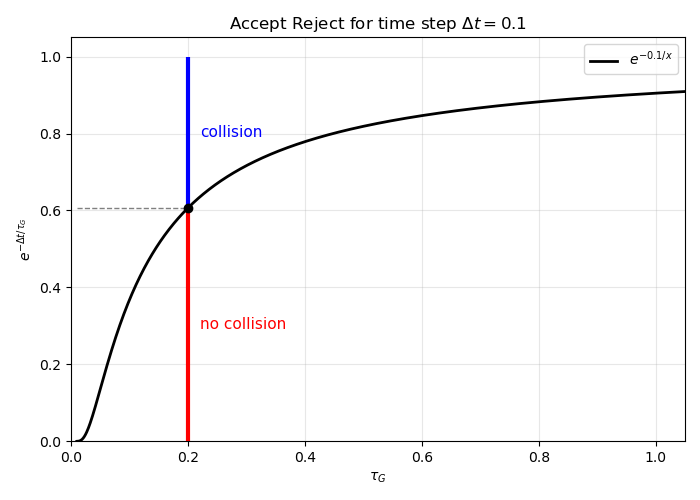
\includegraphics[width=0.7\linewidth]{sections/OpenFOAM/acceptReject.png}
    \caption{Example for a time step $\Delta \tvar = 0.1$ for different damping times.}
    \label{fig:colNoCol}
\end{figure}

If the code determines that a collision has taken place an updated velocity is drawn from a Gaussian distribution centered around the mean velocity $\overline{\up}$
\begin{equation*}
    G(\up ; \overline{\up}, \sigma^2(\m)) = \left(\dfrac{2}{3} \pi \sigma^2(\m)\right)^{-\frac{3}{2}} \operatorname{exp} [-(\up - \overline{\up})/(2/3\sigma^2(\m)).
\end{equation*}
Afterward, velocities are adjusted for momentum conservation.

\ifcode
\begin{lstlisting}[firstline=140]
     // calculate time scales and pdf exponent
    autoPtr<AveragingMethod<scalar>> exponentAveragePtr
    (
        AveragingMethod<scalar>::New
        (
            IOobject
            (
                IOobject::scopedName(this->owner().name(), "exponentAverage"),
                this->owner().db().time().timeName(),
                mesh
            ),
            this->owner().solution().dict(),
            mesh
        )
    );
    AveragingMethod<scalar>& exponentAverage = exponentAveragePtr();
    exponentAverage =
        exp
        (
          - deltaT
           *this->timeScaleModel_->oneByTau
            (
                volumeAverage,
                radiusAverage,
                uSqrAverage,
                frequencyAverage
            )
        )();

    // random sampling
    for (typename CloudType::parcelType& p : this->owner())
    {
        const tetIndices tetIs(p.currentTetIndices());

        const scalar x = exponentAverage.interpolate(p.coordinates(), tetIs);

        if (x < rndGen.sample01<scalar>())
        {
            const vector r(sampleGauss(), sampleGauss(), sampleGauss());

            const vector u = uAverage.interpolate(p.coordinates(), tetIs);
            const scalar uRms =
                sqrt(max(uSqrAverage.interpolate(p.coordinates(), tetIs), 0.0));

            p.U() = u + r*uRms*oneBySqrtThree;
        }
    }

    // correction velocity averages
    autoPtr<AveragingMethod<vector>> uTildeAveragePtr
    (
        AveragingMethod<vector>::New
        (
            IOobject
            (
                IOobject::scopedName(this->owner().name(), "uTildeAverage"),
                this->owner().db().time().timeName(),
                mesh
            ),
            this->owner().solution().dict(),
            mesh
        )
    );
    AveragingMethod<vector>& uTildeAverage = uTildeAveragePtr();
    for (typename CloudType::parcelType& p : this->owner())
    {
        const tetIndices tetIs(p.currentTetIndices());
        uTildeAverage.add(p.coordinates(), tetIs, p.nParticle()*p.mass()*p.U());
    }
    uTildeAverage.average(massAverage);

    autoPtr<AveragingMethod<scalar>> uTildeSqrAveragePtr
    (
        AveragingMethod<scalar>::New
        (
            IOobject
            (
                IOobject::scopedName(this->owner().name(), "uTildeSqrAverage"),
                this->owner().db().time().timeName(),
                mesh
            ),
            this->owner().solution().dict(),
            mesh
        )
    );
    AveragingMethod<scalar>& uTildeSqrAverage = uTildeSqrAveragePtr();
    for (typename CloudType::parcelType& p : this->owner())
    {
        const tetIndices tetIs(p.currentTetIndices());
        const vector uTilde = uTildeAverage.interpolate(p.coordinates(), tetIs);
        uTildeSqrAverage.add
        (
            p.coordinates(),
            tetIs,
            p.nParticle()*p.mass()*magSqr(p.U() - uTilde)
        );
    }
    uTildeSqrAverage.average(massAverage);

    // conservation correction
    for (typename CloudType::parcelType& p : this->owner())
    {
        const tetIndices tetIs(p.currentTetIndices());

        const vector u = uAverage.interpolate(p.coordinates(), tetIs);
        const scalar uRms =
            sqrt(max(uSqrAverage.interpolate(p.coordinates(), tetIs), 0.0));

        const vector uTilde = uTildeAverage.interpolate(p.coordinates(), tetIs);
        const scalar uTildeRms =
            sqrt
            (
                max(uTildeSqrAverage.interpolate(p.coordinates(), tetIs), 0.0)
            );

        p.U() = u + (p.U() - uTilde)*uRms/max(uTildeRms, SMALL);
    }

\end{lstlisting}
\fi

\Todo{Adjust velocity einfügen}
\Todo{$\tilde{u}_{p,i}$ einfügen}



\Todo{damping zeit einfügen}


Lastly cell occupancy is again calculated which will be used to calculate the fluid volume fraction in the next step.
The forces are turned back on for the calculations of the Eulerian grid.

This can be observed in the code below.

\ifcode
\begin{lstlisting}[firstnumber=176,caption= motion from  MPPICCloud/MPPICCloud.C]
    template<class CloudType>
template<class TrackCloudType>
void Foam::MPPICCloud<CloudType>::motion
(
    TrackCloudType& cloud,
    typename parcelType::trackingData& td
)
{
    // Kinematic
    // ~~~~~~~~~

    // force calculation and tracking
    td.part() = parcelType::trackingData::tpLinearTrack;
    CloudType::move(cloud, td, this->db().time().deltaTValue());


    // Preliminary
    // ~~~~~~~~~~~

    // switch forces off so they are not applied in corrector steps
    this->forces().setCalcNonCoupled(false);
    this->forces().setCalcCoupled(false);


    // Damping
    // ~~~~~~~

    if (dampingModel_->active())
    {
        if (this->mesh().moving())
        {
            FatalErrorInFunction
                << "MPPIC damping modelling does not support moving meshes."
                << exit(FatalError);
        }

        // update averages
        td.updateAverages(cloud);

        // memory allocation and eulerian calculations
        dampingModel_->cacheFields(true);

        // calculate the damping velocity corrections without moving the parcels
        td.part() = parcelType::trackingData::tpDampingNoTrack;
        CloudType::move(cloud, td, this->db().time().deltaTValue());

        // correct the parcel positions and velocities
        td.part() = parcelType::trackingData::tpCorrectTrack;
        CloudType::move(cloud, td, this->db().time().deltaTValue());

        // finalise and free memory
        dampingModel_->cacheFields(false);
    }
    

    // Packing
    // ~~~~~~~

    if (packingModel_->active())
    {
        if (this->mesh().moving())
        {
            FatalErrorInFunction
                << "MPPIC packing modelling does not support moving meshes."
                << exit(FatalError);
        }

        // same procedure as for damping
        td.updateAverages(cloud);
        packingModel_->cacheFields(true);
        td.part() = parcelType::trackingData::tpPackingNoTrack;
        CloudType::move(cloud, td, this->db().time().deltaTValue());
        td.part() = parcelType::trackingData::tpCorrectTrack;
        CloudType::move(cloud, td, this->db().time().deltaTValue());
        packingModel_->cacheFields(false);
    }


    // Isotropy
    // ~~~~~~~~

    if (isotropyModel_->active())
    {
        // update averages
        td.updateAverages(cloud);

        // apply isotropy model
        isotropyModel_->calculate();
    }


    // Final
    // ~~~~~

    // update cell occupancy
    this->updateCellOccupancy();

    // switch forces back on
    this->forces().setCalcNonCoupled(true);
    this->forces().setCalcCoupled(this->solution().coupled());
}

\end{lstlisting}
\fi



\subsubsection{coupled}
\ifcode
\begin{lstlisting}
    if (solution_.coupled())
        {
            cloud.relaxSources(cloud.cloudCopy());
        }
\end{lstlisting}
\fi
Here the code checks if the solver is coupled. Since the \MP method is coupled the following code is executed.
\ifcode
\begin{lstlisting}
    template<class CloudType>
void Foam::KinematicCloud<CloudType>::relaxSources
(
    const KinematicCloud<CloudType>& cloudOldTime
)
{
    this->relax(rhokTrans_(), cloudOldTime.rhokTrans(), "rhok");
    this->relax(UTrans_(), cloudOldTime.UTrans(), "U");
    this->relax(UCoeff_(), cloudOldTime.UCoeff(), "U");
}
\end{lstlisting}
\fi
This reduces numerical instabilities to to the old fields being used and prevents abrupt changes between time steps.
The new cloud properties are scalled by $\alpha$ while the old cloud properties are scaled by $(1- \alpha)$
\begin{equation*}
    new = \alpha new + (1- \alpha ) old
\end{equation*}
The default, used in the \MP method is to use $\alpha = 1$. 
\todo{hab niergends relaxation gefunden, wird nicht verwendet?}

Here 
\MP is coupled
\subsubsection{postEvolve}
The \lstinline|postEvolve| function is the counterpart of the \lstinline|preEvolve| function. Previously cashed function are released. This includes the Eulerina fields. Cloud properties as such as the particle positions are written out as needed and the iteration advanced. In line boundary and wall interactions are finalized.
\ifcode
\begin{lstlisting}[firstline=266, caption=KinematicCloud.C]
template<class CloudType>
void Foam::KinematicCloud<CloudType>::postEvolve
(
    const typename parcelType::trackingData& td
)
{
    Log_<< endl;

    if (debug)
    {
        this->writePositions();
    }

    this->dispersion().cacheFields(false);

    this->patchInteraction().postEvolve();

    forces_.cacheFields(false);

    functions_.postEvolve(td);

    solution_.nextIter();

    if (this->db().time().writeTime())
    {
        outputProperties_.writeObject
        (
            IOstreamOption
            (
                IOstreamOption::ASCII,
                this->db().time().writeCompression()
            ),
            true
        );
    }

    if (this->dampingModel().active())
    {
        this->dampingModel().cacheFields(false);
    }
    if (this->packingModel().active())
    {
        this->packingModel().cacheFields(false);
    }
}    
\end{lstlisting}
\fi


\subsection{Interpolation}
\ifcode
\begin{lstlisting}
        const volScalarField& thetaField = kinematicCloud.theta();
    
        alphac = max(1.0 - kinematicCloud.theta(), alphacMin);
        
        alphac.correctBoundaryConditions();
        
        alphacf = fvc::interpolate(alphac);
        
        alphaPhic = alphacf*phic;
        
        fvVectorMatrix cloudSU(kinematicCloud.SU(Uc));
        volVectorField cloudVolSUSu
        (
            IOobject
            (
                "cloudVolSUSu",
                runTime.timeName(),
                mesh
            ),
            mesh,
            dimensionedVector(cloudSU.dimensions()/dimVolume, Zero),
            fvPatchFieldBase::zeroGradientType()
        );

        cloudVolSUSu.primitiveFieldRef() = -cloudSU.source()/mesh.V();
        cloudVolSUSu.correctBoundaryConditions();
        cloudSU.source() = Zero;



\end{lstlisting}
\fi
This calculates the particle volume fraction and uses this to calculate the fluid volume fraction
\begin{equation*}
    \fvf = \max (1-\pvf,\fvf_{min})
\end{equation*}
with $\fvf_{min}$ as a user defined input. This is used to prevent overpacking in cells that could lead to numerical instabilities.
Boundary conditions are corrected.
\lstinline|fvc::interpolate(alphac)| interpolates the fluid volume fraction previously calculated to the Eulerian mesh.
In \lstinline|system/fvSchemes| the interpolation scheme is defined as linear. 
The interpolation used by \OF is the barycentric interpolation.
For the interpolation the cells are divided into tetrahedrons. In the \MP method we use linear interpolation functions
\begin{align*}
    N_1 (x,y,z) &= 1-x-y-z \\
    N_2 (x,y,z) &= x \\
    N_3 (x,y,z) &= y \\
    N_4 (x,y,z) &= z 
\end{align*}

\Todo{interpolation in OpenFOAM}
The effective flux is calculated as \lstinline|alphaPhic| by accounting for the particle effect.
The calculated velocity of the kinematic cloud is used in the momentum source term. This is later used in the \lstinline|PIMPLE| loop.
%SU explicit part, Sp implicit part second part to get per volume


\subsection{Continous Phase, \texttt{PIMPLE} loop}
For the continuous phase, we use the \lstinline|PIMPLE| algorithm for coupling the pressure and the velocity conservation equations.
The name as well as the algorithm is a combination of the \lstinline|PISO| (Pressure Implicit with Splitting of Operator) algorithm with the \lstinline|SIMPLE| (Semi-Implicit Method for Pressure-Linked Equations) algorithm.
In each time step we create two linear matrix systems and solve for the velocity and pressure fields.
The systems are defined in \lstinline|UcEqn| and \lstinline|pEqn|.
For the momentum exchange term between the particles and the fluid the solid force is split up into the explicit and implicit part.
The implicit part \lstinline|cloudSU| is added in \lstinline|UcEqn| and the explicit part  in \lstinline|pEqn|.y

In \lstinline|UcEqn| we start with the momentum equation omitting the pressure term and looking only at the coupled forces
\begin{equation*}
    \dfrac{\partial}{\partial \tvar} (\fvf \uf) + \nabla \cdot (\fvf \phi_f \uf)   -  \left(\dfrac{\partial}{\partial \tvar} \fvf + \nabla \cdot (\phi_f) \right) \uf + S_{turbulence} = \dfrac{1}{\rf} S_{u,exp}
\end{equation*}
The turbulence is set to \lstinline|laminar| in the standard \MP method.
The term subtracted from the equation is zero because of the continuity equation
\begin{equation*}
    \dfrac{\partial}{\partial \tvar} \fvf + \nabla \cdot (\fvf \uf) = 0
\end{equation*}
% fvm::ddt(alphac, Uc) + fvm::div(alphaPhic, Uc)
%   - fvm::Sp(fvc::ddt(alphac) + fvc::div(alphaPhic), Uc)
%   + continuousPhaseTurbulence->divDevRhoReff(Uc)
%  ==
%     (1.0/rhoc)*cloudSU

In \OF these equations are rewritten as
\begin{align*}
    A \uf = b 
\end{align*}
Next relax is called which limits the change that can occur from the previous iteration to the current iteration. Since we do not specify a relaxation factor this has no effect here. Relax also ensures that the matrix $A$ is diagonal dominant, ensuring convergence. 
Before we include the pressure term we define the non-coupled forces for the flux as
\begin{equation*}
    F_{\phi_c} = \left( \dfrac{1}{\rf}A^{-1} S_{u,impl} \right)_{v \to f} + (A^{-1})_{v \to f} (\g \cdot n)
\end{equation*}

Lastly we add the pressure terms and solve
\begin{equation*}
    A \uf -b = F_{\phi_c}(A^{-1})_{v \to f}^{-1} - \nabla \cdot \p A
\end{equation*}
for a first approximation of the velocity.





%minus because of continuity equation


%with the continuous face flux $\phi_f$ and the implicit momentum exchange source term $S_u$
\todo{flux einfach $ \uf$ in Zellinnerem und uA an Boundary, gravity in Source term?}

Flux corrector 
Next we look at the non-coupled forces
\begin{itemize}
    \item $rAUc = (1/UcEqn.A())$ -> .A: invert $A$
    \item surfaceScalarField rAUcf("Dp", fvc::interpolate(rAUc)); interpolieren von cell centers zu cell boundaries
    \item surfaceScalarField phicForces
(
   fvc::flux(rAUc*cloudVolSUSu/rhoc) + rAUcf*(g \& mesh.Sf())
   Gleichung lösen
   \begin{equation*}
       \dfrac{A^{-1} S_{Su}}{\rf} + (A^{-1})|_f (g A)
   \end{equation*}
   with $n$ the normal vector on the corresponding face. With \lstinline|fvf::flux| we once again have the values at cell center.
\end{itemize}

Lastly in \lstinline|UcEqn.C| we include the pressure term and solve the equation

%The flux is for compressible solvers rho*u*A or otherwise u*A on the faces


% volScalarField rAUc(1.0/UcEqn.A());
% surfaceScalarField rAUcf("Dp", fvc::interpolate(rAUc));

% surfaceScalarField phicForces
% (
%    fvc::flux(rAUc*cloudVolSUSu/rhoc) + rAUcf*(g & mesh.Sf())
% );

% UcEqn
%      ==
%         fvc::reconstruct
%         (
%             phicForces/rAUcf - fvc::snGrad(p)*mesh.magSf()
%         )
\begin{equation*}
    A\uf - b=\dfrac{(\dfrac{rAUc S_{Su}}{\rf} + rAUc_f (g \cdot n))|_{cell-centers}}{rAUcf} - (\nabla p)|_f A_f
\end{equation*}
which is called the momentum predictor and is solved for $\uf$.



% PisoFoam solves the momentum equation once each time-step and afterwards does the correction to satisfy continuity.
% If nOuterLoop is zero in PIMPLEFoam we have a PisoFOAM solver. PIMPLEFoam just iterates over it



In the \lstinline|pEqn| file the \lstinline|PISO| loop is executed.


\url{https://doc.cfd.direct/notes/cfd-general-principles/the-pimple-algorithm} how the PIMPLE algorithm works.
The \PIMP algorithm is called in the following loop
\ifcode
\begin{lstlisting}[caption=from MPPICFoam.C]
 while (pimple.loop())
        {
            #include "UcEqn.H"

            // --- PISO loop
            while (pimple.correct())
            {
                #include "pEqn.H"
            }

            if (pimple.turbCorr())
            {
                continuousPhaseTurbulence->correct();
            }
        }

        runTime.write();

        runTime.printExecutionTime(Info);
    }
\end{lstlisting}
\fi


\ifcode
\FloatBarrier
\begin{lstlisting}[caption=UcEqn.H]
    fvVectorMatrix UcEqn
(
    fvm::ddt(alphac, Uc) + fvm::div(alphaPhic, Uc)
  - fvm::Sp(fvc::ddt(alphac) + fvc::div(alphaPhic), Uc)
  + continuousPhaseTurbulence->divDevRhoReff(Uc)
 ==
    (1.0/rhoc)*cloudSU
);

UcEqn.relax();

volScalarField rAUc(1.0/UcEqn.A());
surfaceScalarField rAUcf("Dp", fvc::interpolate(rAUc));

surfaceScalarField phicForces
(
   fvc::flux(rAUc*cloudVolSUSu/rhoc) + rAUcf*(g & mesh.Sf())
);

if (pimple.momentumPredictor())
{
    solve
    (
        UcEqn
     ==
        fvc::reconstruct
        (
            phicForces/rAUcf - fvc::snGrad(p)*mesh.magSf()
        )
    );
}

\end{lstlisting}
\FloatBarrier
\fi
\ifcode
\begin{lstlisting}[caption=pEqn.H]
{
    volVectorField HbyA(constrainHbyA(rAUc*UcEqn.H(), Uc, p));

    surfaceScalarField phiHbyA
    (
        "phiHbyA",
        (
           fvc::flux(HbyA)
         + alphacf*rAUcf*fvc::ddtCorr(Uc, phic)
        )
    );

    if (p.needReference())
    {
        adjustPhi(phiHbyA, Uc, p);
    }

    phiHbyA += phicForces;

    // Update the pressure BCs to ensure flux consistency
    constrainPressure(p, Uc, phiHbyA, rAUcf);

    // Non-orthogonal pressure corrector loop
    while (pimple.correctNonOrthogonal())
    {
        fvScalarMatrix pEqn
        (
            fvm::laplacian(alphacf*rAUcf, p)
         ==
            fvc::ddt(alphac) + fvc::div(alphacf*phiHbyA)
        );

        pEqn.setReference(pRefCell, pRefValue);

        pEqn.solve(p.select(pimple.finalInnerIter()));

        if (pimple.finalNonOrthogonalIter())
        {
            phic = phiHbyA - pEqn.flux()/alphacf;

            p.relax();

            Uc = HbyA
              + rAUc*fvc::reconstruct((phicForces - pEqn.flux()/alphacf)/rAUcf);
            Uc.correctBoundaryConditions();
        }
    }
}

#include "continuityErrs.H"

\end{lstlisting}
\fi




The \texttt{PIMPLE} 





\begin{itemize}
\item For Lagrangian \url{https://openfoamwiki.net/index.php/OpenFOAM_guide/UML/lagrangian}

\end{itemize}


% \section{Comparison Goldschmidt and GoldschmidtMPICC}
% \subsection{Goldschmidt}
% \subsubsection{Geometry}
% \begin{itemize}
%     \item Cuboid with side length of $15mm \ \times \ 150mm \ \times \ 450mm$
%     \item 2,30,90 grading
%     \item 
%     \begin{figure}
%         \centering
%         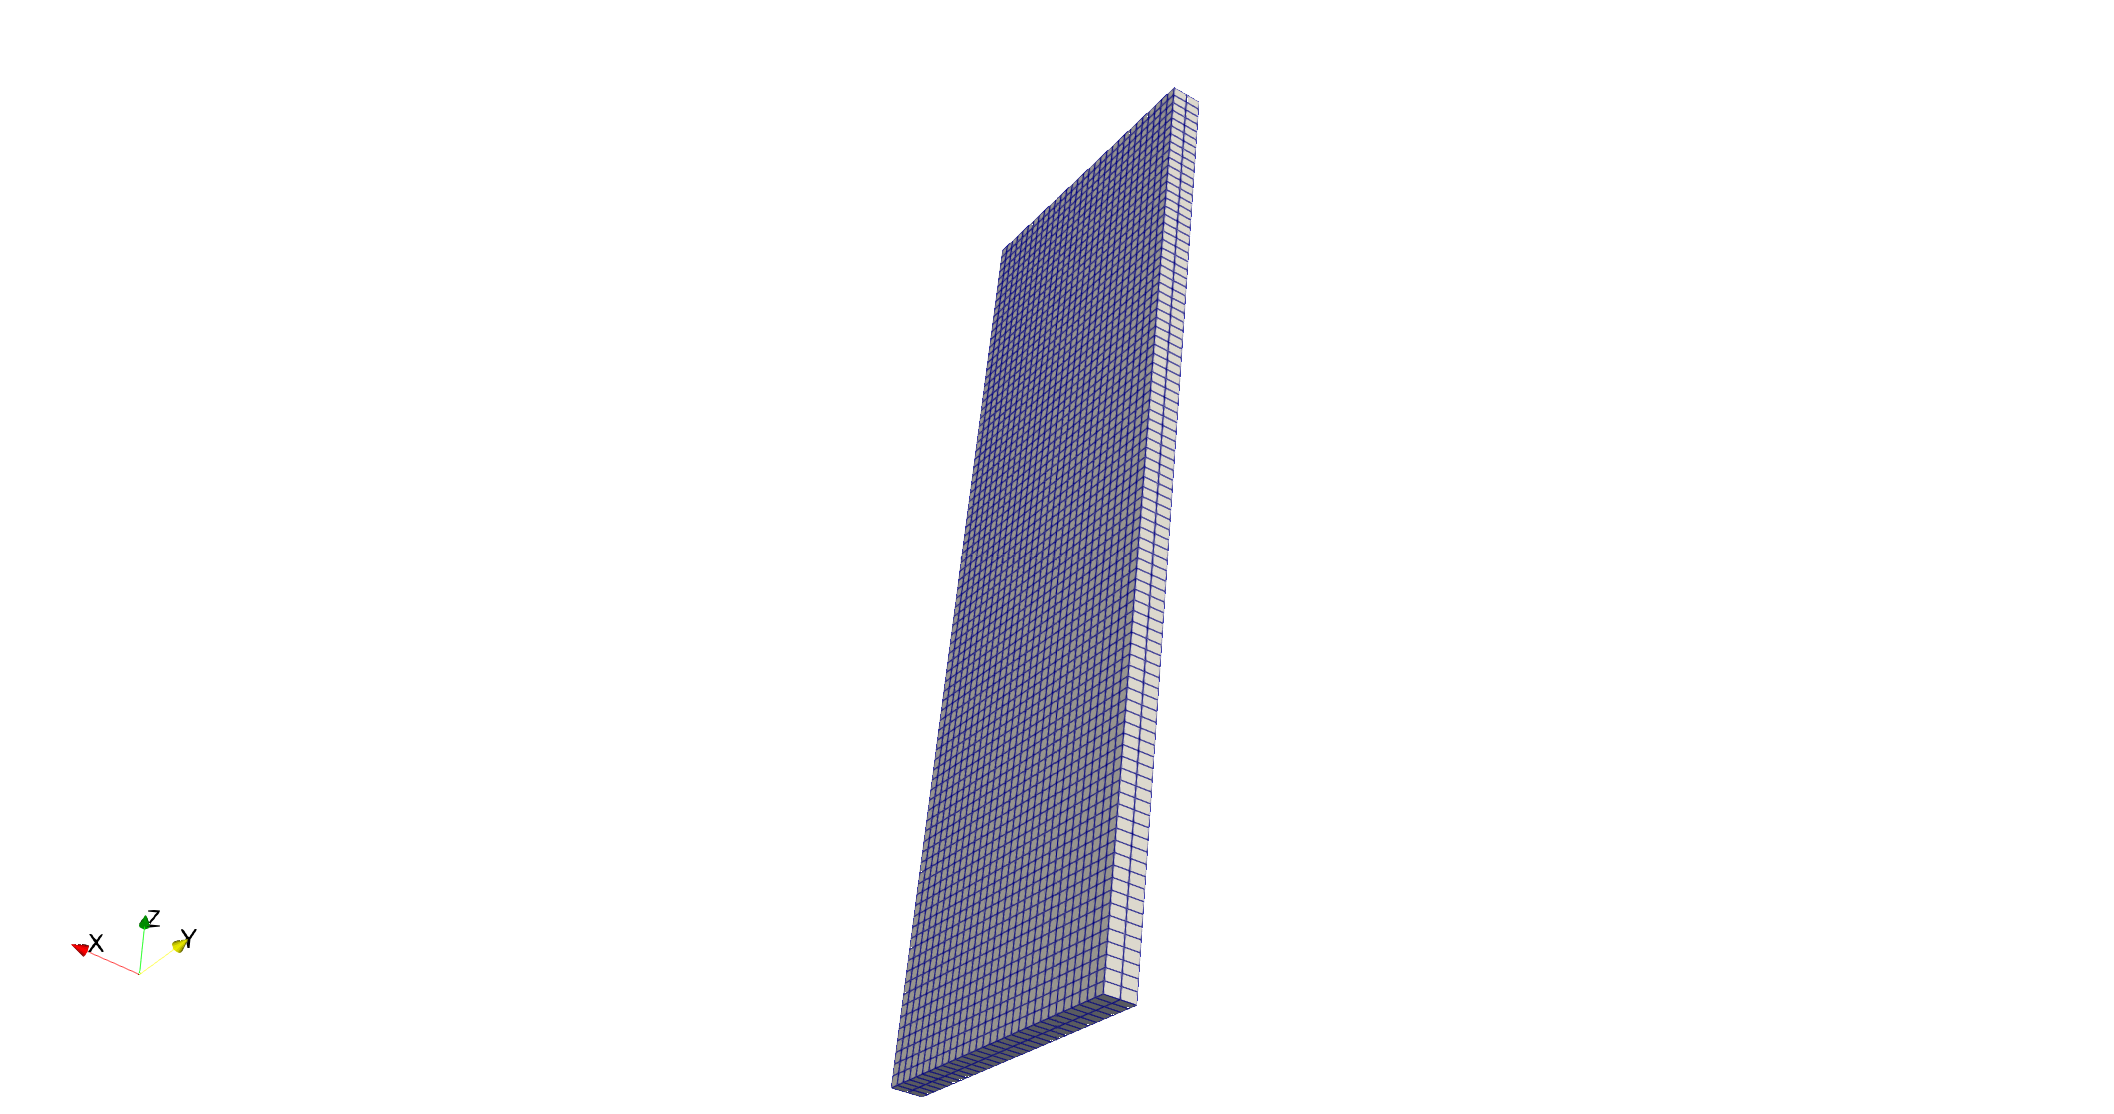
\includegraphics[width=0.8\linewidth]{sections/OpenFOAM/geometry_goldschmidt.png}
%         \caption{Caption}
%         \label{fig:enter-label}
%     \end{figure}
%     \item Top has \texttt{pressureInletOutletVelocity}: zerogrdient condition for outflow velocity with specified inlet direction
%     \item Bottom has \texttt{interstitialInletVelocity}sepecifies inlet velocity field with local phase-fraction
%     \item walls have \texttt{noSlip} fixes velocity to zero at walls
%     \item for pressure look at kinematic pressure: physical pressure/fluidDensity, unit $m²/s²$
%     \item top: \texttt{fixedValue}
%     \item bottom: \texttt{fixedFluxPressure} set pressure gradient to provide value, correct flux at fixed-flux boundaries by compensating for the body forces with the pressure gradient
%     \item front,back: symmetry (same as velocity)
%     \item walls: \texttt{noSlip}
% \end{itemize}
% \subsection{Initial Setup}
% \begin{itemize}
%     \item 24750 particles are distributed equally in five layers
%     \begin{figure}
%         \centering
%         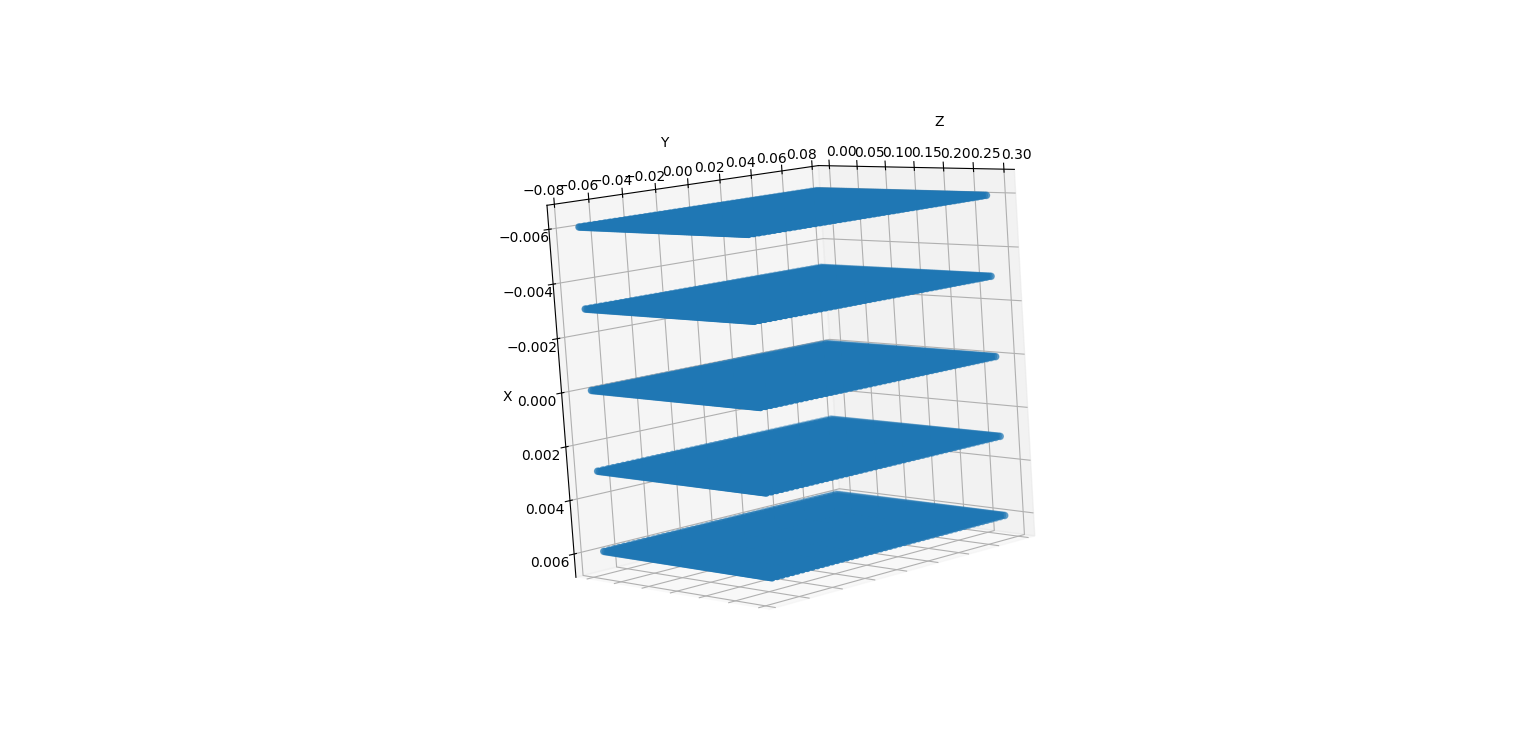
\includegraphics[width=0.5\linewidth]{sections/OpenFOAM/cloud_particle_initial.png}
%         \caption{Caption}
%         \label{fig:enter-label}
%     \end{figure}
%     \item highest z: 0.2955
% \end{itemize}

% \subsubsection{Cloud properties}
% \begin{itemize}
%     \item Difference between both methods: the cloudProperties are of different types
%     \item Classic has type \texttt{collidingCloud}
%     \item collidingCloud: Lagragian cloud class
%     \item for MPPIC: Multi-Phase Particle In Cell  modeling is used to represent collisions without resolving particle-particle interactions
% \end{itemize}
